\section{Information Flow in DGNs}\label{sec:expressivity}
\textbf{Paths:} In a fully connected DGN, $d$ layers and $w$ hidden units per layer, we have a total of $P=d_{in}w^{(d-1)}$ paths. Let us say that an enumeration of the paths is given by $[P]=\{1,\ldots,P\}$. Let $\I_{l},l=0,\ldots,d-1$ provide the index of the hidden unit through which a path $p$ passes in layer $l$ (with the convention that $\I_d(p)=1,\forall p\in [P]$). We then define:\\
$1.$ The value of a path $p$ by $v_t(p)\stackrel{def}=\Pi_{l=1}^d \Theta_t(l,\I_{l-1}(p),\I_l(p))$.\\
$2.$ The activity of a path $p$ for an input $x\in \R^{d_{in}}$ by $A_{t}(x,p)\stackrel{def}{=}\Pi_{l=1}^{d-1} G_{x,t}(l,\I_l(p))$.\\
\textbf{Value Derivative:} For a path $p$, the derivative of its value with respect to any weight in the path is: 
\begin{align}\label{eq:vft}{\partial v_t(p)}/{\partial \Theta\left(l,\I_{l'-1}(p),\I_{l'}(p)\right)}|_{\Theta=\Theta_t}= \underset{l=1}{\underset{l\neq l'}{\overset{d}{\Pi}}} \Theta_t\left(l,\I_{l-1}(p),\I_{l}(p)\right)
\end{align}
If a path $p$ does not pass through a $\theta\in\Theta$, then ${\partial v_t(p)}/{\partial \theta}=0$.\\
\textbf{Activity Derivative:} For a path $p$, and an input $x\inrdin$ the derivative of its activity with respect to any weight is given by 
\begin{align}
\frac{\partial A_{t}(x,p)}{\partial \tg}= \sum_{l=1}^{d-1} \Big(\frac{\partial G_{x,\Tg_t}(l,\I_l(p))}{\partial \tg} \Big)\Big(\Pi_{l'\neq l} G_{x,\Tg_t}(l',I_{l'}(p))\Big)
\end{align}
\begin{lemma}\label{lm:disentangle}[Disentanglement]
Under \Cref{assmp:init}, $\forall\,\theta\in\Theta$, for paths $p,p'\in [P], p\neq p'$:  i) $E{\partial_{\theta}v_0(p)\partial_{\theta}v_0(p')}= 0$ and ii)$\E{\partial_{\theta}v^2_0(p)}= \sigma^{2(d-1)}$, iii) $\E{v_0(p)v_0(p')}=0$, iv) $\E{v^2_0(p)}=\sigma^{2d}$.
\end{lemma}
\begin{comment}
\begin{table}
\begin{minipage}{0.5\columnwidth}
%\resizebox{\columnwidth}{!}{
\begin{tabular}{|c|l|}\hline								 								 													
NPF		&$\phi_{x,t}=(x(\I_0(p))A_t(x,p) ,p\in[P])\in \R^P$\\\hline	
NPK		&$H_t(x,x')=\ip{\phi_{x,t},\phi_{x',t}}$\\\hline		
OAP		&$\lambda_t(x,x')=\sum_{p\rsa i} A_t(x,p) A_t(x',p)$\\\hline
VTP		&$\varphi^v_{p,t}=(\partial_{\theta}v_t(p),\theta\in\Theta)\inrdnet$ \\\hline	
ATP		&$\varphi^a_{x,p,t}=(\partial_{\tg}A_t(x,p),\tg\in\Tg)\inrdnet$ \\\hline	
\end{tabular}
%}
\end{minipage}
\hspace{15pt}
\begin{minipage}{0.5\columnwidth}
%\resizebox{\columnwidth}{!}{
\begin{tabular}{|c|l|}\hline								 								 													
OSP 	&$\delta_t(x,x')=\sum_{p\rsa i} \ip{\varphi^a_{x,p,t},\varphi^a_{x',p,t}}$\\\hline
VG		&$\psi^v_{x,t}=\nabla_{\Theta} \hat{y}_t(x)\in\R^{d_{net}}$\\\hline
AG		&$\psi^{\phi}_{x,t}=\nabla_{\Tg} \hat{y}_t(x)\in\R^{d_{net}}$\\\hline
NTF		&$\psi_{x,t}=(\psi^v_{x,t},\psi^{\phi}_{x,t})\in\R^{2d_{net}}$\\\hline
NTK 		&$K_t(x,x')=\psi^\top_{x,t}\psi_{x',t}$\\\hline
\end{tabular}
%}
\end{minipage}
\caption{Shows all zeroth-order and first-order quantities related to information flow in a DGN.}
\label{tb:terms}
\end{table}
\end{comment}
\subsection{Neural Path Feature and Kernel}
The \emph{neural path feature} of an input example $x_s\in \R^{d_{in}}$ is given by $\phi_{x_s,\G_t}=(x_s(\I_0(p))A_t(x_s,p) ,p\in[P])\in\R^P$. Here, for a path $p$, $\I_0(p)$ is the input node at which the path starts and $A_t(x_s,p)$ is its activation level. By arranging the NPF of the $n$ input examples in a matrix $\Phi_t=\left[\phi_{x_1,t},\ldots, \Phi_{x_n,t}\right]$, we can express the predicted output of a DGN as: 
\begin{align}\label{eq:npfbasic}
\hat{y}_t=\Phi_t^\top v_t,
\end{align}
where, the value of the path $v_t$ is the equivalent of the so called \emph{weight-vector} in a standard linear approximation. 
The significance of the NPF are:\hfill\\
$1.$ \textbf{Signal-Wire Separation}: Note that $\Phi$ encodes the signal: say for a DNN with ReLU activations, the co-ordinate corresponding to path $p$ is either $x(\I_0(p))$ if the path is active for that input (i.e., $A_t(x,p)=1$) or $0$ if the path is inactive for that input  (i.e., $A_t(x,p)=0$). The value of the path thus encodes the \emph{wire}, i.e., the information contained in the weights of the network. \hfill\\
$2.$ \textbf{Deep Information Propagation:} The path view provides a novel way of looking at information propagation in DNNs, eschewing the conventional `layer-by-layer' expression for information flow.\hfill\\
As associated with the NPF matrix is the \emph{neural path kernel} matrix, given by $H_t=\Phi^\top_t\Phi_t$. 
\begin{definition}\label{def:lambda}
$\lambda_t(s,s')\stackrel{def}{=}\sum_{p\rsa i} A_t(x,p) A_t(x',p)$, $\forall s,s'\in[n]$, any $i\in [d_{in}]$,  
 \end{definition} 
\begin{lemma}\label{lm:npk}[Neural Path Kernel] 
Let $x=(x_s,s\in [n])\in\R^{d_{in}\times n}$ be the data matrix and let the neural path kernel matrix be defined as $H_t\stackrel{def}=\Phi^\top_t\Phi_t$. It follows that $H_t= (x^\top x)\odot(\lambda_t)$. 
\end{lemma}
\textbf{NPFs and Optimisation:} The ability of DNNs to fit data has been demonstrated in the past \cite{ben}, i.e., they can fit even random labels, and random pixels of standard datasets such as MNIST. However, for standard DNNs with ReLU gates, with no bias parameters, a dataset with $n=2$ points namely $(x,1)$ and $(2x,-1)$ for some $x\in \R^{d_{in}}$ cannot be memorised. The reason is that the gating values are the same for both $x$ and $2x$ (for that matter any positive scaling of $x$), and hence $\phi_{2x,\G_t }= 2\phi_{x,\G_t }$, and thus it not possible to fit arbitrary values for $\hat{y}_t(x)$ and $\hat{y}_t(2x)$.\\
\textbf{NPFs and Generalisation:} We trained DGN on standard datasets namely MNIST and CIFAR-10, under the following conditions: i) the gates are frozen $\G_t=\G_0,\forall t\geq 0$ and ii) the gating values are obtained from a ReLU network, which acts as the gating network (see \Cref{tb:dgn}). Since, the gates are frozen, the NPFs are fixed and the SGD learns only the path values. We compare the performance of $4$ different NPFs, wherein, the gates are copied from i) from a randomly initialised ReLU network (untrained), ii) from a ReLU network trained with good dataset iii) ReLU network trained on random labels and iv) ReLU network trained on random pixels.
\FloatBarrier
\begin{table}[h]
\begin{tabular}{|c|c|c|c|c|c|c|}\hline
&&&&\multicolumn{3}{c|}{NPF (trained)}\\\cline{5-7}
$(w,d)$	&Dataset		&ReLU		&NPF(untrained) 		&Good 		&Random Labels 	&Random Pixel\\\hline
$(128,6)$	& MNIST 		& $98.15$ 		&$96$ 		&$98.3$		&$92.6$			&$94.3$\\\hline
$(256,6)$	& MNIST 		& $98.5$ 		&$96.6$ 		&$98.4$		&$92.0$			&$81.1$\\\hline
\end{tabular}
\caption{Shows the training and generalisation performance of various GaLU network. Here, non-learned stands for gates from a randomly initialised ReLU network.}
\label{tb:copygate}
\end{table}
\textbf{NPF dynamics:} 
We consider ``Binary''-MNIST data set with two classes namely digits $4$ and $7$, with the labels taking values in $\{-1,+1\}$ and squared loss. We trained a standard DNN with ReLU activation ($w=100$, $d=5$). Recall that $H_t=\Phi^\top_t\Phi_t$  (the Gram matrix of the features) and let $\widehat{H}_t=\frac{1}{trace(H_t)}H_t$ be its normalised counterpart. For a subset size, $n'=200$ ($100$ examples per class) we plot $\nu_t=y^\top (\widehat{H}_t)^{-1} y$, (where $y\in\{-1,1\}^{200}$ is the labeling function), and observe that $\nu_t$ reduces as training proceeds (see first plot in \Cref{fig:gen}). Note that $\nu_t=\sum_{i=1}^{n'}(u_{i,t}^\top y)^2 (\hat{\rho}_{i,t})^{-1}$, where $u_{i,t}\in \R^{n'}$ are the orthonormal eigenvectors of $\widehat{H}_t$ and $\hat{\rho}_{i,t},i\in[n']$ are the corresponding eigenvalues. Since $\sum_{i=1}^{n'}\hat{\rho}_{i,t}=1$, the only way $\nu_t$ reduces is when more and more energy gets concentrated on $\hat{\rho}_{i,t}$s for which $(u_{i,t}^\top y)^2$s are also high. However, in $H_t=(x^\top x)\odot \lambda_t$, only $\lambda_t$ changes with time. Thus, $\lambda_t(s,s')$ which is a measure of overlap of sub-networks active for input examples $s,s'\in[n]$, changes in a manner to reduce $\nu_t$. We can thus infer that the \emph{right} active sub-networks are learned over the course of training. We now summarise the insights obtained from these experiments in the following remarks:\hfill\\
\begin{figure}[h]
\centering
\begin{tabular}{cc}
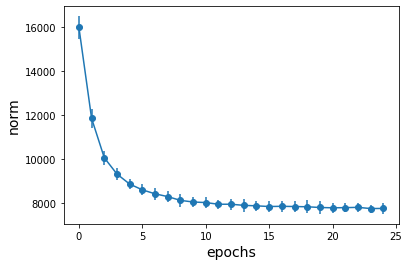
\includegraphics[scale=0.25]{figs/path-gram.png}
&
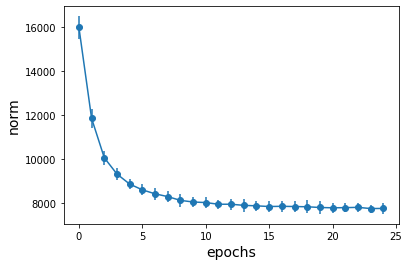
\includegraphics[scale=0.25]{figs/path-gram.png}
\end{tabular}
\caption{First two plots from the left show optimisation and generalisation in ReLU and GaLU networks for standard MNIST. The right most plot shows $\nu_t=y^\top (\widehat{H}_t)^{-1}y$, where $H_t=\Phi_t^\top \Phi_t$.}
\label{fig:gen}
\end{figure}
\section{Prior Art and Gaps: Neural Tangent Feature and Kernel }
The neural tangent features (NTF) is the collection of the output gradients with respect to the network parameters, and is given by $\psi_{x_s,t}=(\nabla_{\Theta|_{\Theta=\Theta_t}} \hat{y}_{\Theta}(x_s))\in\R^{d_{net}}$.  The NTF matrix can be used to linearise the output of a DNN about the point $\Theta_t\inrdnet$. To see this, let the NTF matrix be $\Psi_t=[\psi_{x_1,t},\ldots, \psi_{x_n,t}]\in\R^{d_{net}\times n}$, then a linearisation of the DNN output about $\Theta_t$ is given by:
\begin{align}
\hat{y}_{\Theta_t+\Theta}=\hat{y}_{\Theta_t} + \Psi^\top_t (\Theta-\Theta_t)
\end{align}
An associated \emph{neural tangent kernel} is then given by $K_t=\Psi^\top_t\Psi_t$.\\
\textbf{Optimsation:} \cite{ntk} were the first to point out the role of NTK in DNNs. Using the trajectory based analysis, \cite{dudnn} show that in fully connected DNNs with $w=\Omega(poly(n)2^{O(d)})$, and in residual neural networks (ResNets) with $w=\Omega(poly(n,d))$ gradient descent converges to zero training loss. In the \emph{trajectory} based analysis, one looks at the dynamics of error $e_t$  (i.e., difference between predicted and true values) at time $t$. For a small step-size $\alpha_t>0$, the error dynamics follows a linear recursion given by: $e_{t+1}=e_t-\alpha_tK_te_t$, where $K_t$ is the NTK matrix obtained on the the dataset. Thus, the spectral properties of $K_t$ is key to achieve zero training error. \hfill\\
\textbf{Research Gap I:} The result by \cite{dudnn} shows that ResNets are better than fully connected DNNs, based on the fact that the dependence on the number of layers improves exponentially for ResNets. However, Question I (see \Cref{sec:intro}), i.e., `why depth helps in training?' is unresolved.\\
\textbf{Generalisation:} Prior works by \cite{arora2019exact,cao2019generalization} suggest that, for randomised initialisation, DNNs can be thought of as learning with the linear features given by the random NTFs, and provide generalisation bounds with the corresponding NTK. They use NTK at initialisation to provide generalisation bounds as well as propose pure-kernel methods. However, couple of issues remain unresolved: firstly, if the DNNs are only linear learners with random NTFs, then it suggests that no feature learning happens in DNNs, and secondly, it was observed in prior experiments that the DNNs perform better than their corresponding NTK counterparts \cite{arora2019exact,lee2017deep}. \hfill\\
\textbf{Research Gap II:} However, couple of issues remain unresolved: firstly, if the DNNs are only linear learners with random NTFs, then it suggests that no feature learning happens in DNNs, and secondly, it was observed in prior experiments that the DNNs perform better than their corresponding NTK counterparts \cite{arora2019exact,lee2017deep}.
\section{Bridging the Gap: NTK equals NPK for random initialisation}
In this section, we assume that the NPKs are given to us and fixed (i.e, $G_t=\G_0,\forall t\geq 0$ is given to us). We show that, at randomised weight initialisation, the NTK is equal to (but for a scaling factor) to the NPK. We then use the \emph{Hadamard} structure of the NPK to comment about optimisation and generalisation. 
\begin{assumption}\label{assmp:main}
(i) $\Theta_0\inrdnet$  is statistically independent of $\G_0$ and (ii) The weights $\Theta_0$ are sampled i.i.d from a distribution such that for any $\theta_0\in\{\Theta_0\cup \Tg_0\}$,  we have $\E{\theta_0}=0$, and  $\E{\theta^2_0}=\sigma^2$, and $\E{\theta^4_0}={\sigma'}^2$.
\end{assumption}
\begin{lemma}\label{lm:disentangle}[Disentanglement] Let $\varphi_{p,t}=(\nabla_{\Theta} v_t(p))\inrdnet$, 
under \Cref{assmp:main}-(ii), $\forall\,\theta\in\Theta$, for paths $p,p'\in [P], p\neq p'$:  i) $\E{\ip{\varphi_{p,0},\varphi_{p',0}}}= 0$ and ii)$\E{\ip{\varphi_{p,0},\varphi_{p,0}}}= \sigma^{2(d-1)}$, iii) $\E{v_0(p)v_0(p')}=0$, iv) $\E{v^2_0(p)}=\sigma^{2d}$.
\end{lemma}
\begin{theorem}\label{th:main} Under \Cref{assmp:main}, we have:\\
(i) $\E{K_0}=\sigma^{2(d-1)}H_0=\sigma^{2(d-1)}(x^\top x)\odot(\lambda_0)$,\\
(ii) In addition, if ${4d}/{w^2}<1$, then $Var\left[K^v_0\right]\leq O\left(d^2_{in}\sigma^{4(d-1)}\max\{d^2w^{2(d-2)+1}, d^3w^{2(d-2)}\}\right)$,\\
\end{theorem}
\textbf{Active Sub-Network and Gradient Flow:}  Each input example has its own associated set of active sub-network, and while training a particular example, the gradient flows through the weights of the corresponding active sub-network. Now, the active sub-networks corresponding to different examples have some overlap, and hence there is bound to be \emph{cross-talk} of the gradients flowing through them. This overlap is captured by $\lambda_t(s,s')$ which is the measure of overlap of the sub-networks that are active for both the inputs $x,x'\in\R^{d_{in}}$. As seen from \Cref{th:main}, $\lambda_0$ directly controls the spectral properties of the NTK matrix $K_0$. Formally put, let $\varphi_t=(\varphi_{p,t},p\in[P])\in \R^{d_{net}\times P}$ matrix, then since $K_t=\Psi^\top_t\Psi$, where $\Psi_t=\varphi_t \Phi_t$, we have $\E{K_t}=\E{\Phi^\top_t \varphi^\top_t \varphi_t \Phi_t}$. At initialisation, using the \Cref{assmp:main}-(i), we can pull out $\Phi^\top_t$ and $\Phi_t$ outside of the expectation to have
$\E{K_0}=\Phi^\top_0\E{ \varphi^\top_t \varphi_t }\Phi_0$, and from \Cref{lm:disentangle}, it follows that $\E{ \varphi^\top_t \varphi_t }=d\sigma^{2(d-1)}I$.

\textbf{Optmisation: The role of depth}\\
$\bullet$\textbf{Why increasing depth till a point helps in training? } From \Cref{th:main}-(ii) it follows that for $w\ra\infty$, $K_0\ra\E{K_0}$. We now argue that when $\sigma=\sqrt{\frac{2}{w}}$, increasing depth causes whitening of $\lambda_0$, and hence $K_0$ .\hfill\\
$1.$ Let us first look at the diagonal terms of $\lambda_0$. It is reasonable to assume that, owing to the symmetric nature of the weights, roughly $\mu=\frac{1}{2}$ fraction of the gates are \emph{on} every layer. Thus $\lambda_0(s,s)\approx (w/2)^{d-1}$. Now, due our choice of $\sigma=\sqrt{\frac{2}{w}}$, the diagonal entries will be close to $1$.\hfill\\
$2.$ We now turn our attention towards the non-diagonal entries of $\lambda_0$. Define $\tau(s,s',l)\stackrel{def}=\sum_{i=1}^w G_{x_s,t}(l,i)G_{x_{s'},t}(l,i)$ be the overlap of the active gates in layer $l$ for input examples $s,s'\in[n]$, and  let $\eta\stackrel{def}=\max_s\left(\max_{s',l} \frac{\tau(s,s',l)}{\tau(s,s,l)}\right)$ be the maximum overlap between gates of a layer (maximum taken over over input pairs $s,s'\in[n]$ and layers $l\in [d]$).  Then it follows that $\max_{s,s'\in [n]} \frac{\bar{\lambda}_{cross}(s,s')}{\bar{\lambda}_{self}(s)}\leq \eta^{d-1}$. Thus, the non-diagonal entries decay an exponential rate in comparison to the diagonal entries.\hfill\\
\textbf{Why increasing the depth beyond hurts training?} Note that for $\sigma=O\left(\sqrt{\frac{1}{w}}\right)$, for a fixed depth $d$, as width $w$ increases, $K_0\ra\E{K_0}$. However, the variance expression in \Cref{th:main}-$(ii)$ involves $d^2$ and $d^3$ terms, and hence for a fixed width as depth increases, the entries of $K_0$ deviates from $\E{K_0}$, and as a result the spectrum of $K_0$ degrades, thereby hurting training performance.
\textbf{Generalisation: Role of Feature Learning}\\
As seen before in our experiments that, different NPFs give different generalisation performance, and that NPF/NPK is learnt during training. In this light, a missing link in results by \cite{arora2019exact,cao2019generalization}, is that NTKs are completely dependent on gating.
\subsection{Fixed random gating: Explicit spectrum for NPK} 
Consider the dataset $(x_s,y_s)_{s=1}^n\in \R\times \R$, where $x_s=1,\forall s\in [n]$, and $y_s\sim unif([-1,1])$, $n=200$. The input Gram matrix $x^\top x$ is a $n\times n$ matrix with all entries equal to $1$ and its rank is equal to 1. Since all the inputs are identical, this is the worst possible case for optimisation. In this experiment, since we are interested only in the optimisation question, we take full control of the gating. For each input example, we sample gating values from $Ber(\mu)$ taking values in $\{0,1\}$, and collect it in $\G_0$. In this case, it is easy to check that $\mathbf{E}_{\mu}\left[\lambda_0(s,s)\right]=(\mu w)^{(d-1)},\forall s\in[n]$ and $\mathbf{E}_{\mu}\left[\lambda_0(s,s')\right]=(\mu^2 w)^{(d-1)},\forall s,s'\in[n]$.\hfill\\
\textbf{Theoretical Prediction:} It follows that,  for $\sigma=\sqrt{\frac{1}{\mu w}}$, all the diagonal entries of $\E{K_0}/d$ are $1$ and non-diagonal entries are $\mu^{d-1}$. Now, let $\rho_i\geq 0,i \in [n]$ be the eigenvalues of $\frac{\E{K_0}}{d}$, and let $\rho_{\max}$ and $\rho_{\min}$ be the largest and smallest eigenvalues.  One can easily show that $\rho_{\max}=1+(n-1)\mu^{d-1}$ and corresponds to the eigenvector with all entries as $1$, and $\rho_{\min}=(1-\mu^{d-1})$ repeats $(n-1)$ times, which corresponds to eigenvectors given by $[0, 0, \ldots, \underbrace{1, -1}_{\text{$i$ and $i+1$}}, 0,0,\ldots, 0]^\top \in \R^n$ for $i=1,\ldots,n-1$.\hfill\\
\begin{figure*}
\resizebox{\textwidth}{!}{
\begin{tabular}{ccc}
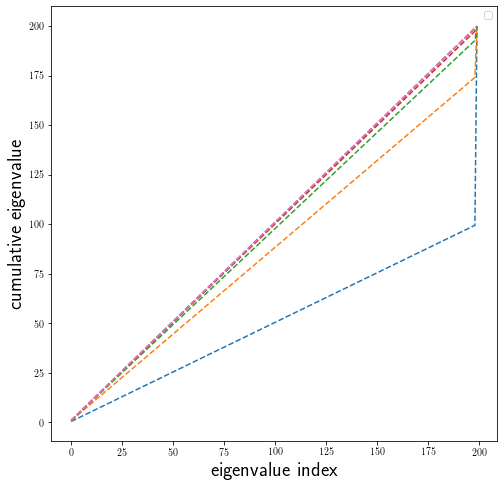
\includegraphics[scale=0.4]{figs/dgn-fra-ecdf-ideal.png}
&
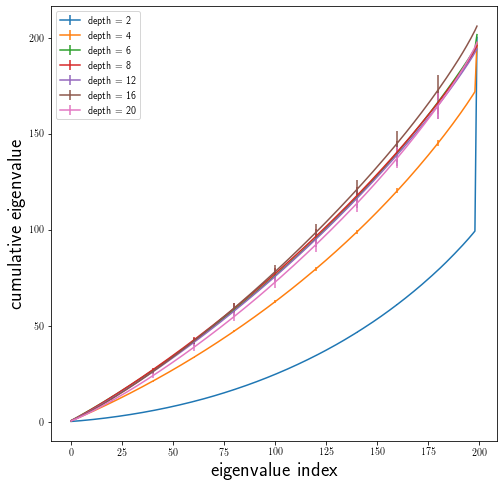
\includegraphics[scale=0.4]{figs/dgn-fra-ecdfbyd-w500.png}
&
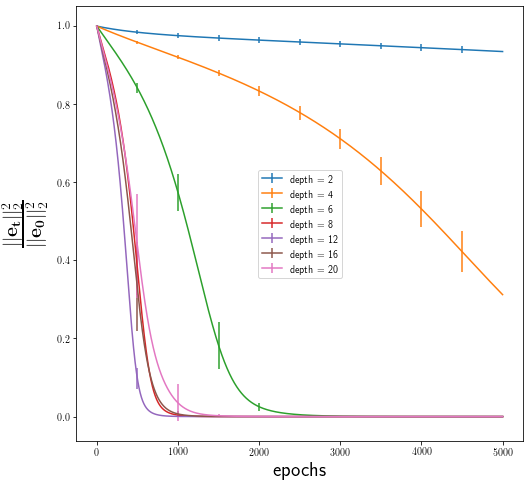
\includegraphics[scale=0.4]{figs/dgn-fra-conv-w500.png}
\end{tabular}
}
\caption{Shows the plots for DGN-FRG with $\mu=\frac{1}{2}$ and $\sigma=\sqrt{\frac{2}{w}}$. The first plot in the left shows the ideal cumulative eigenvalue (e.c.d.f) for various depths $d=2,4,6,8,12,16,20$. Note that the ideal plot converges to identity matrix as $d$ increases. The second plot from the left shows the cumulative eigenvalues (e.c.d.f) for $w=500$. }
\label{fig:dgn-frg-gram-ecdf}
\end{figure*}
\textbf{Numerical Evidence:} We look at the cumulative eigenvalue (e.c.d.f) obtained by first sorting the eigenvalues in ascending order then looking at their cumulative sum. The ideal behaviour (middle plot of \Cref{fig:dgn-frg-gram-ecdf}) as predicted from theory is that for indices $k\in[n-1]$, the e.c.d.f should increase at a linear rate, i.e., the cumulative sum of the first $k$ indices is equal to $k(1-\mu^{d-1})$, and the difference between the last two indices is $1+(n-1)\mu^{d-1}$. In \Cref{fig:dgn-frg-gram-ecdf}, we plot the e.c.d.f for various depths $d=2,4,6,8,12,16,20$ and $w=500$. \hfill\\
In order to compare how the rate of convergence varies with the depth, we set the step-size $\alpha=\frac{0.1}{\rho_{\max}}$, $w=100$. We use the vanilla SGD-optimiser. Note that the convergence rate is determined by a linear recursion $e_{t+1}=e_t-\alpha_t K_te_t$, and choosing $\alpha=\frac{0.1}{\rho_{\max}}$ can be seen to be equivalent to having a constant step-size of $\alpha=0.1$ but dividing the Gram matrix by its maximum eigenvalue instead. Thus, after this rescaling, the maximum eigenvalue is $1$ uniformly across all the instances, and the convergence should be limited by the smaller eigenvalues. We also look at the convergence rate of the ratio $\frac{\norm{e_t}^2_2}{\norm{e_0}^2_2}$, and we observe that the convergence rate gets better with depth as predicted by theory.
\section{Feature Learning}
Consider a parameterised DGN, and given a dataset $(x_s,y_s)_{s=1}^n\in \R^{d_{in}}\times \R$, let $\Phi_{\Theta}=(\phi_{x_s,\Theta},s\in[n] )\in \R^{P\times n}$ be the NPF matrix  $y=(y_s,\in[n])\in\R^n$ be the vector of target values to be learnt, and say we are interested in minimising the square loss given by:
\begin{align}\label{eq:sqloss}
\min_{\Theta\in \R^{d_{net}}, \Tg\in \R^{d_{net}}}\norm{\Phi_{\Tg}v_{\Theta}-y}^2_2
\end{align}
A gradient descent update for the above objective in \eqref{eq:sqloss} involves two gradient components, namely: \\
(i) The value gradient $\psi^v_{x,t}=\nabla_{\Theta} \hat{y}_t(x)\in\R^{d_{net}}$, which learns the values keeping the NPF fixed.\\
(ii) The feature gradient $\psi^{\phi}_{x,t}=\nabla_{\Tg} \hat{y}_t(x)\in\R^{d_{net}}$, which learns the NPFs keeping the values fixed.\\
In order to gain insight into this the joint optimisation and feature learning, we consider the following toy experiment.\\
\textbf{A Toy Experiment:} We look at a simple neural network with $d_{in}=2$, $w=2$ and $1$-hidden layer (see first diagram on the left in \Cref{fig:feat}). The first layer weights is an identity matrix, and for input $x\in\R^2$ to the network, the first layer output is given by $z_{t}(i)=x(i)G_t(i),i=1,2$, where $G_t(i)=\frac{1}{1+\exp(-\tg(i))},i=1,2$. In this network, there are $2$ paths, and the NPF is given by $\phi_{x,t}=(x(1)G_t(1),x(2)G_t(2))\in \R^2$ (note that this mimics the general structure of the NPF as presented in \Cref{sec:expressivity}).
We check the performance of frozen-gates versus adaptable gates in this network. We consider a binary classification task, with $n=500$ example for each class, with class $+1$ and $-1$ examples sampled from $U([0.1,1]\times [-a,a])$ and $U([-1,-0.1]\times[-a,a])$ respectively. We considered two cases $a=1$ (first two plots from the left in \Cref{fig:feat}), and $a=100$ (right most plot in \Cref{fig:feat}). 
We trained the simple neural network using gradient descent with step-size of $0.1$, initialisation $\Tg_0=\Theta_0=(0,0)\in\R^2$, and binary cross entropy loss for the following two cases: i) frozen-gates, wherein, we set $\Tg_0=\Tg_t=\Tg_0,\forall t\geq 0$, and train only $\Theta_t$ ii) adaptable gates, wherein, we train both $\Tg_t$ and $\Theta_t$. In all the plots, green bold and black dotted lines corresponds to classifier learned  by adaptable and frozen gates respectively, and the points are represented using the NPF.
%While both cases train for $T=10^4$ epochs, for $T=10^3$ epochs only the model with adaptable gates trains successfully. The results are shown in \Cref{fig:feat}, notice that the right most plot shows that in the case when the gates are adapting, they learn to suppress the second co-ordinate (the scale of $\phi_{x_s,T}$ is from $-15$ to $15$ as opposed to $-100$ to $100$ in $x_s$).
\FloatBarrier
\begin{figure}[h]
\begin{minipage}{0.15\columnwidth}
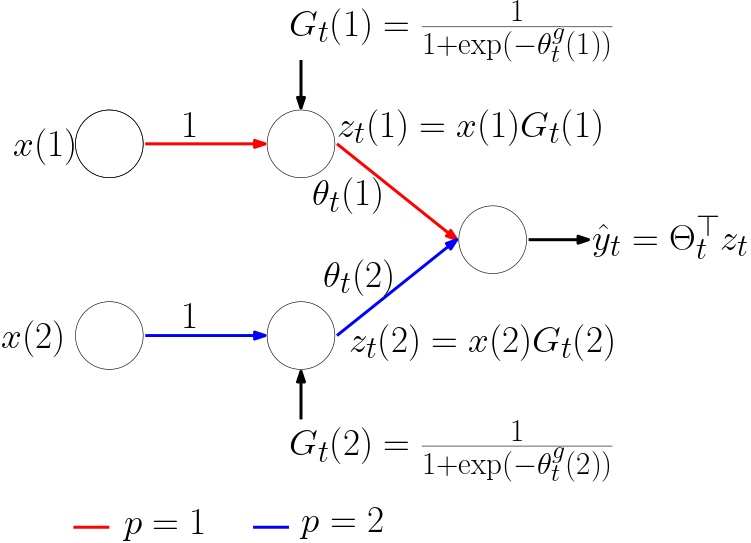
\includegraphics[scale=0.15]{figs/featlearn.png}
\end{minipage}
\hspace{50pt}
\begin{minipage}{0.8\columnwidth}
\resizebox{1\columnwidth}{!}{
\begin{tabular}{cccc}
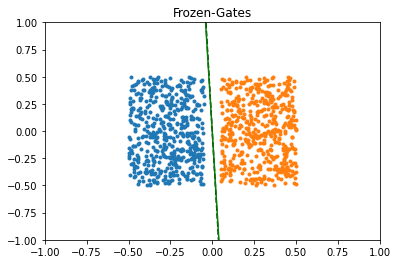
\includegraphics[scale=0.2]{figs/simple-1e2.png}
&
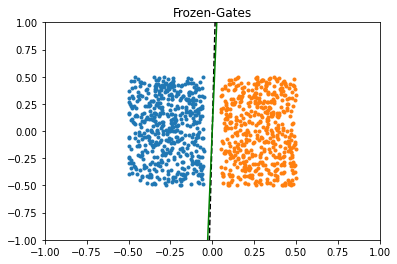
\includegraphics[scale=0.2]{figs/simple-1e3.png}
&
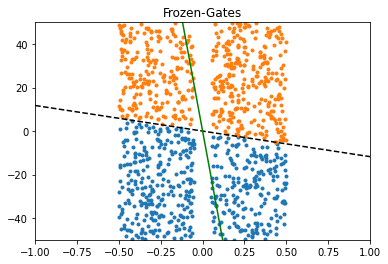
\includegraphics[scale=0.2]{figs/simple.png}
&
%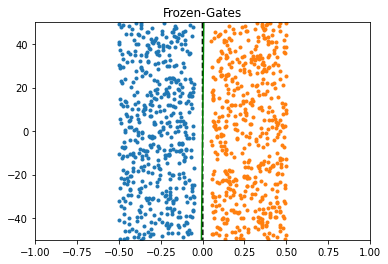
\includegraphics[scale=0.2]{figs/simple-1e4.png}
\\
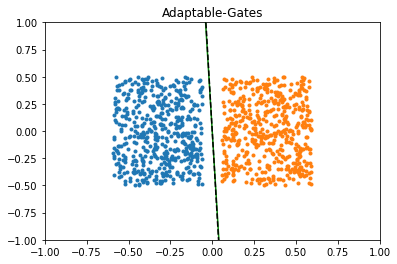
\includegraphics[scale=0.2]{figs/adapt-1e2.png}
&
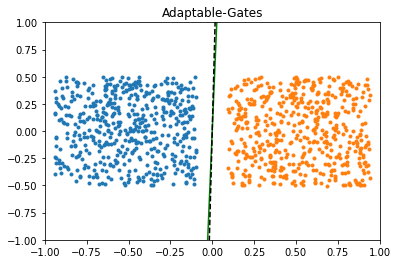
\includegraphics[scale=0.2]{figs/adapt-1e3.png}
&
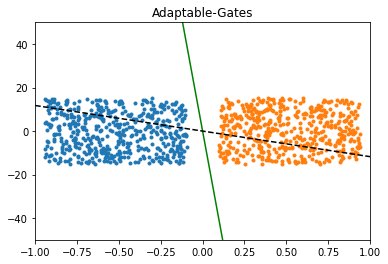
\includegraphics[scale=0.2]{figs/adapt.png}
&
%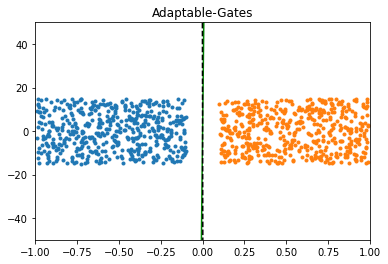
\includegraphics[scale=0.2]{figs/adapt-1e4.png}
\end{tabular}
}
\end{minipage}

\caption{From left: second and third plots shows the training performance of frozen and adaptable gates respectively. In both plots, the bold line in green is the classifier learnt in the case of adaptable gates, and the dotted black line is the classifier learnt in the case of frozen gates. Notice the transformation of the feature space in the case of adaptable gates.}
\label{fig:feat}
\end{figure}
\textbf{Observations:}\\
$1.$ Initially for both networks $\tg_0=(0,0)^\top$, which means the horizontal and vertical co-ordinates in the NPF are both scaled by a factor of $0.5$. For the case of $a=1$, both networks train successfully in $T=10^2$ epochs, and we do not see any change in the NPFs. However, when trained for $T=10^3$ epochs, the network with adaptable gates learns to scale the horizontal co-ordinate in the NPF by factor $1.0$, while it retains a value of $0.5$ for the vertical co-ordinate (see second plot from left of \Cref{fig:feat}).\\
$2.$ In the case of $a=100$ (right-most plot), the adaptable network successfully trains in $T=10^3$ epochs by learning to scale the vertical co-ordinate down by a factor close to $0.15$. However, the network with frozen-gates does not train. We also observed that both networks trained successfully for $T=10^4$ epochs.
%\textbf{An open question:} Informally speaking, in the above example, even though the gating parameters had $2$-degrees of freedom, it was nonetheless sufficient to adapt the features. Thus, perhaps we can hypothesise that subject to the `well-conditioned' ness of $K^a_t$, such margin increase can be perhaps achieved for all the $n$ examples.  However, in practice, both $\Tg_t$ as well as $\Theta_t$ change, and an open question is to understand how the joint optimisation and feature learning happens. 

\begin{comment}
\textbf{Zeroth-order feature and kernel:} We now introduce the \emph{neural path feature} (NPF) and the \emph{neural path kernel} (NPK), which are zeroth-order quantities defined using the gating information $\G_t$. These quantities hold for all kinds of networks namely ReLU, GaLU, soft-ReLU and soft-GaLU. \\
The NPF of an input $x\in \R^{d_{in}}$ is given by $\phi_{x,t}=(x(\I_0(p))A_t(x,p) ,p\in[P])\in\R^P$. By arranging the NPF of the $n$ input examples in a matrix $\Phi_t=\left[\phi_{x_1,t},\ldots, \Phi_{x_n,t}\right]$, we can express the predicted output of a DGN as: \begin{align}\label{eq:npfbasic}\hat{y}_t=\Phi_t^\top v_t,\end{align}
where, the value of the path $v_t$ is the equivalent of the so called \emph{weight-vector} in a standard linear approximation. 

The significance of the NPF are:\hfill\\
$1.$ \textbf{Signal-Wire Separation}: Note that $\Phi$ encodes the signal: say for a DNN with ReLU activations, the co-ordinate corresponding to path $p$ is either $x(\I_0(p))$ if the path is active for that input (i.e., $A_t(x,p)=1$) or $0$ if the path is inactive for that input  (i.e., $A_t(x,p)=0$). The value of the path thus encodes the \emph{wire}, i.e., the information contained in the weights of the network. \hfill\\
$2.$ \textbf{Deep Information Propagation:} The path view provides a novel way of looking at information propagation in DNNs, eschewing the conventional `layer-by-layer' expression for information flow.\hfill\\
$3.$ \textbf{Representation:} As a parallel to the standard linear approximation, the NPF can be regarded as the \emph{hidden feature} and $v_t$ as the weight vector.
\end{comment}
\begin{comment}
$\lambda_t(s,s')$ is to be understood as the measure of overlap of the sub-networks that are active for both the inputs $x,x'\in\R^{d_{in}}$. Note that the definition of $\lambda_t$ is independent of $i\in [d_{in}]$: owing to symmetry the same number of paths start from any given input node, and looking forward, the paths see exactly the same gates and gating values in the subsequent layers.

%\subsection{First-order feature and kernel}
\textbf{Activity Derivative:} For a path $p$, and an input $x\inrdin$ the derivative of its activity with respect to any weight is given by 
\begin{align}
\frac{\partial A_{t}(x,p)}{\partial \tg}= \sum_{l=1}^{d-1} \Big(\frac{\partial G_{x,\Tg_t}(l,\I_l(p))}{\partial \tg} \Big)\Big(\Pi_{l'\neq l} G_{x,\Tg_t}(l',I_{l'}(p))\Big)
\end{align}
\end{comment}

\begin{comment}
Given that the output of a DGN is expressed as $\hat{y}_t(x)=\phi_{x,t}^\top v_t$, we define the following:\\
$1.$ \textbf{Value gradient:} $\psi_{x,t}^v=(\nabla_{\Theta}v_t)^\top  \phi_{x,t}$, which learns the value of the paths keeping the NPF fixed. \\
$2.$ \textbf{Feature gradient:}  $\psi_{x,t}^{\phi}=(\nabla_{\Tg}\phi_{x,t})^\top v_t $, which learns the NPFs keeping the value of the paths fixed. Note that the feature gradient is $0$ in the case of hard-gates.
To the best of our knowledge, for the first time in the literature, we note that the gradient flow has two components. Note that, in the value and feature gradients, quantities $\nabla_{\Theta}v_t$ and $\nabla_{\Tg}\phi_{x,t}$ are $P\times d_{net}$ matrices, which are obtained by computing the derivative of $v_t(p)$ and $\phi_{x,t}(p)$ for all paths $p\in[P]$ with respect to the respective $d_{net}$ parameters.\\
\end{comment}

\begin{comment}
\textbf{Neural Tangent Feature (NTF):} $\psi_{x,t}=[\psi^v_{x,t},\psi^{\phi}_{x,t}]\in \R^{2d_{net}}$. \\
\textbf{Neural Tangent Kernel (NTK):} $K_t(x,x')=K^v_t(x,x')+K^{\phi}_t(x,x')$, where $K^v_t(x,x')={\psi^v}^\top_{x,t}\psi^v_{x',t}$ and $K^{\phi}_t(x,x')={\psi^{\phi}}^\top_{x,t}\psi^{\phi}_{x',t}$. 
\begin{assumption}\label{assmp:decouple}
$\G_0$ is statistically independent of $\Theta_0\inrdnet$ or in the case of parameterised gating, $\Tg_0\inrdnet$ is statistically independent of $\Theta_t\inrdnet$.
\end{assumption}
\end{comment}

\begin{definition}\label{def:delta}
$\delta_t(x,x')\stackrel{def}= \underset{{p\rsa i}}{\sum} \sum_{\tg\in\Tg}\frac{\partial A_{t}(x,p)}{\partial \tg} \frac{\partial A_{t}(x',p)}{\partial \tg}$, for $x,x'\in\R^{d_{in}}$, using any $i\in[d_{in}]$.
\end{definition}
Note that in \Cref{def:delta}, $\delta_t$ contains $\partial A_t(x,p)$ terms as opposed to $A_t(x,p)$ term in $\lambda_t$ defined in \Cref{def:lambda}.
\begin{theorem}\label{th:main} Let $x=(x_s,s\in[n])\in \R^{d_{in}\times n}$ be the data matrix. Then, under \Cref{assmp:init,assmp:decouple}, we have:\\
(i) $\E{K_0}=\E{K^v_0}+\E{K^{\phi}_0}$, where $\E{K^{v}_0}=\sigma^{2(d-1)} (x^\top x)\odot \lambda_0$, and $\E{K^{\phi}_0}=\sigma^{2d}  (x^\top x)\odot \delta_0$.\\
(ii) In addition, if ${4d}/{w^2}<1$, then $Var\left[K^v_0\right]\leq O\left(d^2_{in}\sigma^{4(d-1)}\max\{d^2w^{2(d-2)+1}, d^3w^{2(d-2)}\}\right)$,\\
where $K_0, K^v_0, K^{\phi}_0, \lambda_0, \delta_0$ are matrices defined on the dataset.
\end{theorem}

